\documentclass[tikz,border=6pt]{standalone}

% shared cartoon info
\usepackage{xcolor}
\usepackage{siunitx}
\usepackage{tikz}
\usetikzlibrary{calc,arrows.meta,backgrounds}

\newcommand{\Lx}{1}
\newcommand{\Ly}{3}
\newcommand{\Lz}{3}
\newcommand{\R}{0.25} % sphere radius = 1/3 (diameter 2/3)

\def\nuclei{
  0.15/0.60/0.70,
  0.35/1.40/2.50,
  0.75/2.10/1.10,
  0.60/0.90/2.20,
  0.20/2.60/0.50,
  0.90/1.80/1.70
}

\newcommand{\xcut}{0.05}

% Colors (example)
\definecolor{wcprimary}{RGB}{081,040,136}
\definecolor{wcalerted}{RGB}{202,124,027}
\definecolor{wcexample}{RGB}{000,134,086}

\tikzset{
  box/.style      = {line width=0.5pt, draw=black},
  nucleus3D/.style= {draw=black, fill=black!15},
  nucleus2D/.style= {draw=black, fill=black!25},
  beam/.style     = {-{Latex[length=2.2mm,width=1.8mm]},  thick},
  axislabel/.style= {font=\scriptsize},
  yzplane/.style = {fill=black,fill opacity=0.15},
  cutring/.style = {draw=black, dashed, line width=0.5pt, dash pattern=on 2pt off 1.2pt}
}


\begin{document}
  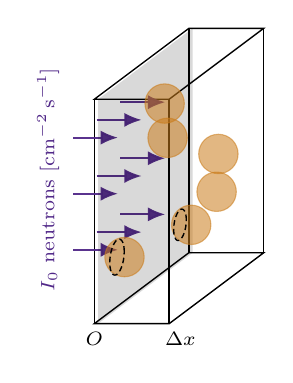
\begin{tikzpicture}[scale=1.,
    % Simple oblique projection: set 3D basis vectors in 2D
    x={(0.95cm, 0cm)}, y={(0.40cm, 0.30cm)}, z={(0cm, 0.95cm)}
  ]
    % Slab (rectangular prism)
    % bottom face z=0
    \draw[box] (0,0,0) -- (\Lx,0,0) -- (\Lx,\Ly,0) -- (0,\Ly,0) -- cycle;
    % top face z=\Lz
    \draw[box] (0,0,\Lz) -- (\Lx,0,\Lz) -- (\Lx,\Ly,\Lz) -- (0,\Ly,\Lz) -- cycle;
    % verticals
    \draw[box] (0,0,0) -- (0,0,\Lz);
    \draw[box] (\Lx,0,0) -- (\Lx,0,\Lz);
    \draw[box] (\Lx,\Ly,0) -- (\Lx,\Ly,\Lz);
    \draw[box] (0,\Ly,0) -- (0,\Ly,\Lz);

    % Parallel beam along +x (a few guide arrows)
    \foreach \yy in {0.75, 1.5, 2.25}{
      \foreach \zz in {0.75, 1.5, 2.25}{
        \draw[beam,opacity=0.95,color=wcprimary] (-0.6,\yy,\zz) -- (0,\yy,\zz);
      }
    }
    \node[axislabel, rotate=90, color=wcprimary] at (-1.25,1.5,1.45) {$I_0$ neutrons [\si{\per\centi\meter\squared\per\second}]};
    
    \path[yzplane]
      (\xcut, 0, 0) -- (\xcut, \Ly, 0) -- (\xcut, \Ly, \Lz) -- (\xcut, 0, \Lz) -- cycle;
    
    
    % Nuclei drawn as circles (same radius for all; orthographic cue)
    \foreach \x/\y/\z in \nuclei {
      \filldraw[nucleus3D, opacity=0.55, color=wcalerted] (\x,\y,\z) circle[radius=\R cm];
    }
    
    \begin{scope}
    \clip (\xcut,0,0) -- (\xcut,\Ly,0) -- (\xcut,\Ly,\Lz) -- (\xcut,0,\Lz) -- cycle;

    \foreach \x/\y/\z in \nuclei {
        \pgfmathsetmacro{\dx}{\x - \xcut}
        \pgfmathsetmacro{\rr}{sqrt(max(0,\R*\R - \dx*\dx))}
        \ifdim \rr pt>0pt
        \draw[cutring, samples=120, domain=0:360, variable=\t, smooth]
            plot ({\xcut}, {\y + \rr*cos(\t)}, {\z + \rr*sin(\t)});
        \fi
    }
    \end{scope}
    
    
    % Axes labels (schematic)
    \node[axislabel] at (0,0,-0.2) {$O$};
    \node[axislabel] at (\Lx+0.15,0,-0.2) {$\Delta x$};
  \end{tikzpicture}
\end{document}
